%% -*- coding: utf-8; -*-

\documentclass[
  master
  brazilian
]{ThesisPUC}


%%%
%%% Additional Packages
%%%

  \usepackage[brazilian]{babel}      %% in ThesisPUC.cls
  %% \usepackage[utf8]{inputenc}        %% .
  %% \usepackage[T1]{fontenc}           %% .
  %% \usepackage{lmodern}               %% .
  %% \usepackage[pdftex]{graphicx}	%% .

  \usepackage{tabularx}
  \usepackage{multirow}
  \usepackage{multicol}
  \usepackage{colortbl}
  \usepackage[%
    dvipsnames,
    svgnames,
    x11names,
    fixpdftex
  ]{xcolor}
  \usepackage{numprint}
  \usepackage{textcomp}
  \usepackage{booktabs}
  \usepackage{amsmath}
  \usepackage{enumitem}
  \usepackage{amssymb}
  \usepackage{textcomp}
% \usepackage{etoolbox}
  \usepackage{float}
  \usepackage[bottom]{footmisc}

%% numprint 
\npthousandsep{.}
\npdecimalsign{,}

%% ThesisPUC option
%\tablesmode{figtab} %% [nada, fig, tab ou figtab]
%\abreviationsmode{none} %% [none ou use] %% Default is [use]


%%%
%%% Counters
%%%

%% uncomment and change for other depth values
%% \setcounter{tocdepth}{3}
%% \setcounter{lofdepth}{3}
%% \setcounter{lotdepth}{3}
%% \setcounter{secnumdepth}{3}


%%%
%%% New commands and other global definitions
%%%

% -*- coding: iso-8859-1; -*-

%%%
%%% Newcommands
%%%

\newcommand{\degree}{\ensuremath{^\circ}}

\newcommand{\cetem}{Centro de Tecnologia Mineral}

\newcommand{\mybulletOB}{%
  % \textbullet
  % \checkmark
  $\triangleright$
  %\textopenbullet
}

\newcolumntype{L}{>{\raggedright \arraybackslash}X}
\newcolumntype{R}{>{\raggedleft \arraybackslash}X}
\newcolumntype{C}{>{\centering \arraybackslash}X}
\newcolumntype{M}[1]{>{\centering\hspace{0pt}}m{#1}}

\newcommand{\mrcel}[2]{%
\begin{tabular}[c]{@{}c@{}}#1\\#2\end{tabular}}

\newcommand{\mrcell}[2]{%
\begin{tabular}[l]{@{}l@{}}#1\\#2\end{tabular}}

\newcommand{\mrcelthree}[3]{%
\begin{tabular}[c]{@{}c@{}c@{}}#1\\#2\\#3\end{tabular}}

\newcommand{\mrcelcolorg}[2]{%
\begin{tabular}{l}\rowcolor{Gainsboro}#1\\#2\end{tabular}}

\newcommand{\mytbcimg}[3]{%
  \multicolumn{1}{C}{\parbox[c]{#1}{\includegraphics[width=#2]{#3}}}}


%%%
%%% Misc.
%%%

\usecolour{true}

%%%
%%% Titulos
%%%

\author{Vinicius da Silva Costa Almada}
\authorR{Almada, Vinicius da Silva Costa}

\advisor{Luiz Fernando Martha}{Prof.}
\advisorR{Martha, Luiz Fernando}
% If the advisor's department is different from author's department, uncomment the next line and type the correct name and acronym of advisor's institution.
%\advisorInst{institution name}{acronym}

\coadvisor{André Luís Müller}{Dr.}
\coadvisorR{Müller, André Luís}
\coadvisorInst{Instituto Tecgraf/PUC-Rio}{Tecgraf/PUC-Rio}

%% \title{Desenvolvimento de um sistema de microscopia digital para
%%  classificação automática de tipos de hematita em minério de ferro}

\title{Mapeamento de Superfícies e Volume Baseado em Restauração de Seções Geológicas}

\titleuk{Surface and Volume Mapping Based on Restoration of Geological Sections}

%% \subtitulo{Aqui vai o subtitulo caso precise}

\day{30}
\month{Junho}
\year{2021}

\city{Rio de Janeiro}
\CDD{XYZ.AB}
\program{Engenharia Civil}
\school{Centro Técnico Científico}
\university{Pontifícia Universidade Católica do Rio de Janeiro}
\uni{PUC-Rio}

%%%
%%% Jury
%%%

\jury{%
  \jurymember{Banca Um}{Prof.}
    {Universidade Federal de Minas Gerais}{UFMG}
  \jurymember{Banca Dois}{Prof.}
    {Universidade Federal de Ouro Preto}{UFOP}
  \jurymember{Banca Três}{Dr.}
    {Centro de Tecnologia Mineral}{CETEM/MCTI}
  \jurymember{Banca Quatro}{Dr.}
    {Departamento de Engenharia Química e de Materiais}{PUC-Rio}
}

%%%
%%% Resume
%%%

\resume{%
  Bacharel em Engenharia Civil pelo Instituto Federal de Educação, Ciência e Tecnologia do Maranhão (IFMA), formou-se em 2018. Foi bolsista de programas de Iniciação Científica PIBITI – IFMA, com projeto de desenvolvimento de software para Mecânica dos Solos e um segundo na área de Dinâmica das Estruturas. Este último foi base para seu Trabalho de Conclusão de Curso, cujo objetivo foi desenvolver um software para análise dinâmica de estruturas sujeitas à carregamento sísmico. Desde o fim de 2019 atua no Instituto Tecgraf como bolsista no Grupo de Modelagem Geológica de Sistemas Petrolíferos}

%%%
%%% Acknowledgment (REMINDER TO SCHOLARSHIP STUDENTS. Do not forget to thank the agencies that supported your work.)
%%%

\acknowledgment{%
  \noindent Primeiro parágrafo de agradecimento ...
  \bigskip

  \noindent Segundo parágrafo de agradecimento ...
}

%%%
%%% Catalog prekeywords
%%%

\catalogprekeywords{%
  \catalogprekey{Engenharia Civil e Ambiental}%
  \catalogprekey{Engenharia}%
}

%%%
%%% Keywords
%%%

\keywords{%
  \key{Geologia Estrutural}
  \key{Mapeamento de Superfícies Geológicas}
  \key{Mapeamento de Volume Geológico}
}

\keywordsuk{%
  \key{Structural Geology}%
  \key{Mapping of Geological Sections}%
  \key{Mapping of Geological Surfaces}%
}

%%%
%%% Abstract
%%%

\abstract{%
  \textit{Ainda é o resumo do pré-projeto}

  Esse projeto visa desenvolver, dentro do Sistema Recon MS, um fluxo de trabalho que envolve as áreas de geologia estrutural, estratigrafia e geologia de reservatórios. Esse fluxo inicia com a restauração de modelos geológicos (seções e superfícies). Dentro do Sistema Recon busca-se aprimorar as ferramentas em seu ambiente de visualização 3D, denominado multi-seções, ou MS. Através de duas formas diferentes serão desenvolvidas ferramentas que irão prover as geometrias para o ambiente de simulação estratigráfica (para cada tempo geológico): 1) mapeamento de litologias e outras propriedades durante a restauração de seções, que por sua vez gerarão os paleo-relevos; 2) restauração de superfícies em si, que elimina a necessidade do mapeamento do item 1. A importância de ambas as estratégias consiste no fato de que nem sempre é possível obter bons resultados com restauração de superfícies, já que os mecanismos de restauração de seções desenvolvidos são muito mais geológicos. Para o mapeamento é necessária a criação de uma estrutura de dados que represente a malha de superfícies com possibilidade de armazenar informações, como propriedades e ligações entre as entidades das superfícies com as seções. Atualmente o Sistema Recon trabalha de forma totalmente desacoplado entre a estruturas de dados que representa as seções geológicas e a estrutura que representa as superfícies geológicas (horizontes, falhas e tipo do sal). Já para a segunda abordagem, ou seja, a restauração de superfícies, prevê-se o desenvolvimento de um módulo computacional de otimização dedicada a eliminar os buracos das superfícies que estão sendo restauradas incluindo restrições de deslocamento, sobre as falhas geológicas, das sub-superfícies abaixo da superfície restaurada.
}

\abstractuk{%
  This project aims to develop, within the Recon MS System, a workflow that involves the areas of structural geology, stratigraphy and reservoir geology. This flow begins with the restoration of geological models (sections and surfaces). The Recon System seeks to improve the tools in its 3D visualization environment, called multi-sections, or MS. Through two different forms, tools will be developed that will provide the geometries for the stratigraphic simulation environment (for each geological time): 1) mapping of lithologies and other properties during the restoration of sections, which in turn will generate paleo-reliefs; 2) surface restoration itself, which eliminates the need for mapping item 1. The importance of both strategies is the fact that it is not always possible to obtain good results with surface restoration, since the section restoration mechanisms developed are much more geological. For mapping, it is necessary to create a data structure that represents the surface mesh with the possibility of storing information, such as properties and links between the entities of the surfaces and the sections. Currently the Recon System works in a totally decoupled way between the data structures that represent the geological sections and the structure that represents the geological surfaces (horizons, faults and salt type). For the second approach, that is, the restoration of surfaces, it is foreseen the development of a computational optimization module dedicated to eliminate the holes of the surfaces that are being restored including displacement restrictions, on the geological faults, of the sub-surfaces below the restored surface.}

%%%
%%% Dedication
%%%

\dedication{%
  Dedicado lorem ipsum
}

%%%
%%% Epigraph
%%%

\epigraph{%
  My beautifull epigraph
}
\epigraphauthor{Wassily Kandinsky}
\epigraphbook{Regards sur le passé}

%%%
%%% Hyphenation
%%%

\hyphenation{PON-TI-FÍ-CIA}

%%%
%%%
%%% Quotes command
\newcommand{\quotes}[1]{``#1''}

%%%
%%% 
%%%

\begin{document}

  % -*- coding: utf-8; -*-

\chapter{Introdução}

This is the first chapter...



  % -*- coding: utf-8; -*-

\chapter{Processo de Restauração de Seções Geológicas}

\section{Sistema Recon MS}

\subsection{Introdução}

O ambiente no qual este trabalho é desenvolvido é o \textit{Sistema Recon MS}, um software amplamente usado dentro da indústria de óleo e gás pela Petrobras e capaz de auxiliar na restauração de modelos geológicas.\cite{ReconTecgraf} Conta com editor gráfico, estruturas de dados topológicos, algoritmos de transformações geológicas, gráficos de pós-processamentos entre outros recursos.

O Sistema Recon é desenvolvido a partir de um convênio entre o Instituto Tecgraf/PUC-Rio e a Petrobras desde 1991. Atualmente sua equipe responsável é formada pelo Grupo de Modelagem Digital em Geociências do Tecgraf. Uma imagem (Figura~\ref{fig-recon}) da tela inicial do programa é mostrada abaixo.

\begin{figure} [H]
  \begin{center}
    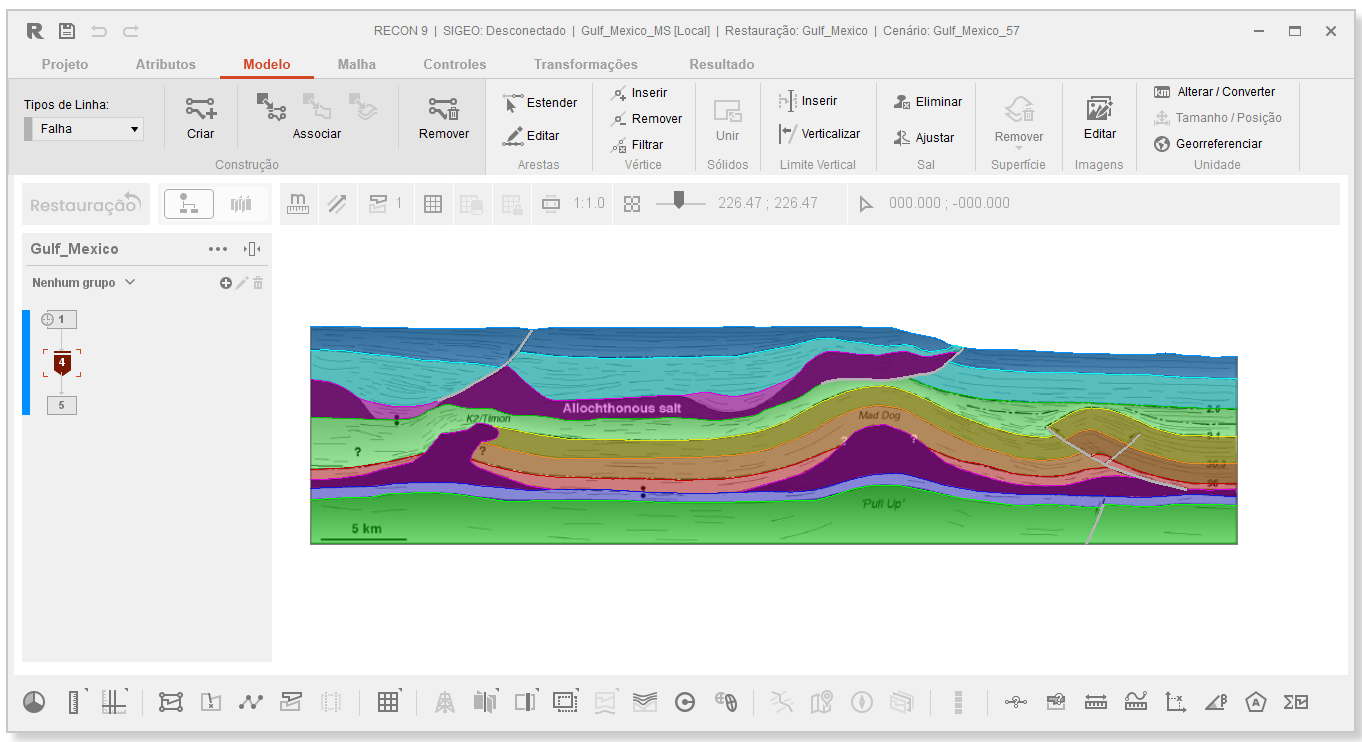
\includegraphics[width=\textwidth]{images/fig-recon}
    \caption{Captura de tela do Sistema Recon MS\cite{Recon}.}\label{fig-recon}
  \end{center}
\end{figure}

A restauração de seções geológicas pode ser entendida como uma manipulação da seção a fim de realizar a reconstituição dela ao seu estado anterior às deformações ocorridas ao longo do tempo, em outras palavras busca-se realizar uma retrodeformação na seção e assim usar na interpretação estrutural de uma região de interesse.\cite{Fossen}

Neste capítulo são apresentadas as principais características do Sistema Recon MS para o objeto deste trabalho a fim de prover uma contextualização para o que é exibido nos demais capítulos. As próximas subseções tratam da descrição dos componentes principais e recursos básicos disponibilizados pelo programa no processo de restauração de seções geológicas e também de visualização tridimensional do modelo. 

\subsection{Subdivisão Planar} % Falar do HED e da TopS

Uma seção geológica pode ter sua representação digital como uma subdivisão planar uma vez que ela pode ser vista como um conjunto de polígonos que dividem o domínio da seção. Estes polígonos podem sofrer deformações e deslocamentos oriundos das transformações geológicos às quais a seção pode sofrer durante o balanceamento. Há ainda informações de adjacências entres essas porções que também precisam ser consideradas em um contexto computacional da seção geológica.

Na Figura~\ref{fig-subdivisao-planar} é possível perceber, por exemplo, que as camadas A, B e C possuem 3 blocos separados por falhas. Cada bloco é uma região fechada delimitada por um conjunto de segmentos. Deve-se observar ainda que essas regiões possuem atributos geológicos como idade, litologia, porosidade, etc.

\begin{figure} [h]
  \begin{center}
    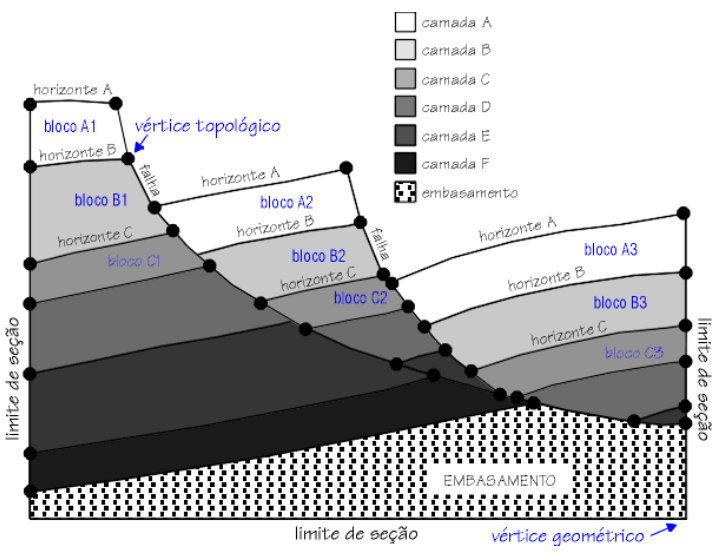
\includegraphics[width=400pt]{images/fig-subdivisao-planar}
    \caption{Seção geológica como uma subdivisão planar.\cite{Ferraz}}\label{fig-subdivisao-planar}
  \end{center}
\end{figure}

Uma subdivisão planar pode ser definida como uma subdivisão do plano através do uso de \textit{arestas}, \textit{vértices} e \textit{faces}.\cite{Berg} Essas são as entidades topológicas presentes em uma subdivisão planar, a face é como a região descrita anteriormente, delimitada por arestas (segmentos de curva); os vértices são os limites das arestas, sendo um para cada extremidade (podendo ser o mesmo vértice no início e no final da aresta).

A subdivisão planar precisa atender a alguns requisitos em relação às entidades topológicas: não deve haver vértices coincidentes; arestas só podem se cruzar em um vértice e faces também só se cruzam ou em um vértice, ou em uma aresta. Em outras palavras, não deve existir sobreposição de elementos topológicos. 

No entanto, há ainda um último componente topológico: o \textit{loop} ou \textit{laço} que é, de forma sucinta, um suconjunto conexo e ordenado de arestas. Com essa definição, a \textit{face} pode ser interpretada como uma união de laços, um deles sendo externo (delimitando a fronteira externa da face) e zero ou mais internos.

Em suma, a subdivisão planar tem os seguintes elementos topológicos:
\renewcommand{\labelitemi}{•}
\begin{itemize}
  \item \textbf{Vértice}: representa um ponto único dentro do plano.
  \item \textbf{Aresta}: segmento de curva com vértices como limites.
  \item \textbf{Laço} (loop): suconjunto conexo e ordenado de arestas.
  \item \textbf{Face}: região delimitada por um ou mais laços.
\end{itemize}

\subsection{Modelagem da Subdivisão Planar}

Para modelar a subdivisão planar dentro do Recon é utilizada a biblioteca computacional \textbf{HED} desenvolvida pelo Instituto Tecgraf/PUC-Rio que é a implementação de uma estrutura de dados topológicos baseada em arestas, a \textit{Half-Edge}, uma das razões para esta escolha são as relações fixas de adjacência que uma aresta apresenta em relação às outras componentes topológicas. Uma aresta sempre é delimitada por dois vértices (distintos ou não) e é adjacente à duas faces.\cite{HED}

O HED introduz uma nova entidade que explora bem essa característica denominada \textit{half-edge} ou \textit{semiaresta} que é uma referência ao \quotes{uso} da aresta por uma face. Dessa forma, no HED, cada aresta é formada por duas semiarestas, cada semiaresta guarda uma referência para uma face e também para um vértice de origem. Isto dá uma orientação para a semiaresta que é usada para indicar o sentido positivo do loop das faces, por exemplo.

A estrutura HED tem um aspecto hierárquico de listas duplamente encadeada de elementos topológicos. No nível mais alto está a subdivisão planar, denominada como \textit{HedSolid}, então vêm \textit{HedFace}, \textit{HedLoop}, \textit{HedHalfEdge} e \textit{HedVtx} no nível mais baixo. A representação da aresta, \textit{HedEdge} encontra-se no mesmo nível da HedHalfEdge.

Uma propriedade importante em estruturas topológicas são as relações de adjacências entre suas componentes, a HED não provê de forma direta todos as relações, contudo é possível chegar às demais com uso de indireções. Por exemplo, partindo de uma aresta, como chegar às faces vizinhas? Basta ir às semiarestas da aresta, cada semiaresta possui referência para uma face.

Apresentado o HED e seus elementos, a associação com as entidades geológicas é intuitiva. Uma camada geológica é representada por uma face; as linhas de horizonte, falha ou sal têm como correspondente as arestas, por último, cada conjunto contínuo de faces é associado a um sólido\footnote{Os sólidos representam uma subdivisão planar e em alguns casos, a seção pode apresentar partes inteiramente descontínuas onde cada uma é um sólido diferente. Para casos onde é necessário sobreposição de partes, só é possível com a existência de mais de um sólido.}.

Destaca-se que a ideia de representar a seção geológica como uma subdivisão planar, ou uma estrutura HED, visa facilitar a criação e manipulação computacional da seção durante o processo de restauração. Todavia, a representação completa precisa levar em consideração também os atributos geológicos.

\subsection{Atributos Geológicos}

Como já dito, os blocos que formam a seção geológica possuem propriedades próprias e precisam também estarem salvas na estrutura de dados topológica.

Cada entidade do HED possui um campo reservado para um tipo genérico de informações e é neste espaço que são organizados os atributos geológicos da seção. Estes atributos são representados em estruturas chamadas \textit{GeoSolid}, \textit{GeoFace}, \textit{GeoEdge} e \textit{GeoVtx}. Pela nomenclatura, é fácil observar a relação com o HED. As principais informações organizadas nessas estruturas são:

\renewcommand{\labelitemi}{•}
\begin{itemize}
  \item \textbf{GeoSolid}: o sólido por ser a estrutura mais alto nível, é quem vai guardar referência à seção e ao cenário ao qual pertence dentro da restauração.
  \item \textbf{GeoFace}: é a estrutura que precisa armazenar dados do material geológico que a compõe (como idade, tipo, características físicas, etc.) e malha de triângulos que pode ser manipulada pelas transformações.
  \item \textbf{GeoEdge}: estrutura que guarda o tipo de linha (de horizonte, falha, topo de sal, etc.) e a subdivisão geométrica que forma a linha. 
  \item \textbf{GeoVtx}: é a única que armazena apenas o identificador universal.
\end{itemize}

Aliás, todas as estruturas de atributos geológicos possuem um campo para salvar este identificador que possui o formato \textit{UUID} --- \textit{universally unique identifier} ou identificador único universal que é usado, por exemplo, na associação dos elementos geológicos com a malha triangular das faces, que será apresentada adiante.\cite{UUID}

\subsection{Seções Geológicas} % Falar da árvore de cenários

O principal recurso do Sistema Recon é seu conjunto de ferramentas para manusear uma seção geológica, desde a digitalização das informações que a definem geometricamente, da caracterização dos materiais e propriedades, da criação de dispositivos de controle e monitoramento da restauração até o kit de transformações que irão deformar a seção.

\subsubsection{Criação de uma seção geológica}

Para criar uma seção geológica no Sistema Recon pode-se recorrer ao editor gráfico para desenhar linhas e atribuir propriedades manualmente conforme seu tipo (se for horizonte, falha, limites da seção, etc.) ou em modelos que apresentem superfícies tridimensionais, como na Figura~\ref{fig-recon-1}, as seções podem ser criadas pela interseção de um plano vertical segundo uma direção dada pelo usuário, essa ação é chamada de \textit{fatiamento} do modelo.

\begin{figure} [H]
  \begin{center}
    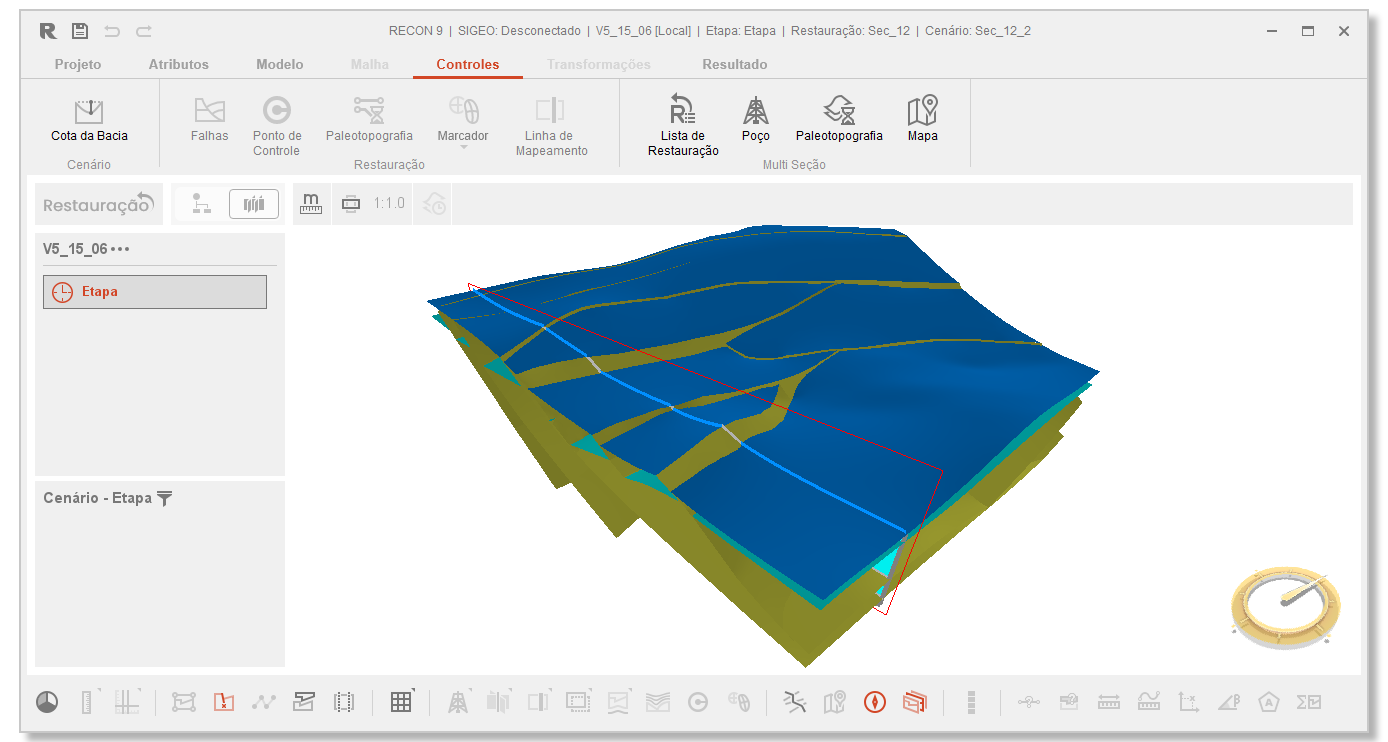
\includegraphics[width=\textwidth]{images/fig-recon-1}
    \caption{Sistema Recon exibindo um modelo com superfícies tridimensionais e uma seção em destaque.}\label{fig-recon-1}
  \end{center}
\end{figure}

Neste último caso, em especial no contexto deste trabalho, o ideal é que após a seção ter sido criada ocorra o mínimo de edição inicial nas linhas geradas. Isso é importante pois quanto melhor definida esteja a seção após o fatiamento, mais coerente com as superfícies tridimensionais estará o modelo como um todo. Edições nas linhas são comuns de acontecerem para que seja possível realizar a restauração da seção. Entretanto, em caso de edições maiores ocorrerá o descasamento entre seção e superfícies, mais tarde, no mapeamento da superfície, poderão haver incongruências.

\subsubsection{Malhas da seção geológica}

A seção geológica é representada como uma subdivisão planar, como já citado, e é utilizada a biblioteca HED na implementação dessa subdivisão. Na Figura~\ref{fig-recon-2} pode-se observar uma seção geológica e alguns elementos, como as linhas (\textit{HedEdges}) onde a sua cor representa o atributo de tipo e as faces (\textit{HedFaces}) que são, em termos simples, regiões fechadas por linhas. Neste exemplo, todas as faces pertencem à mesma camada geológica.

\begin{figure} [h]
  \begin{center}
    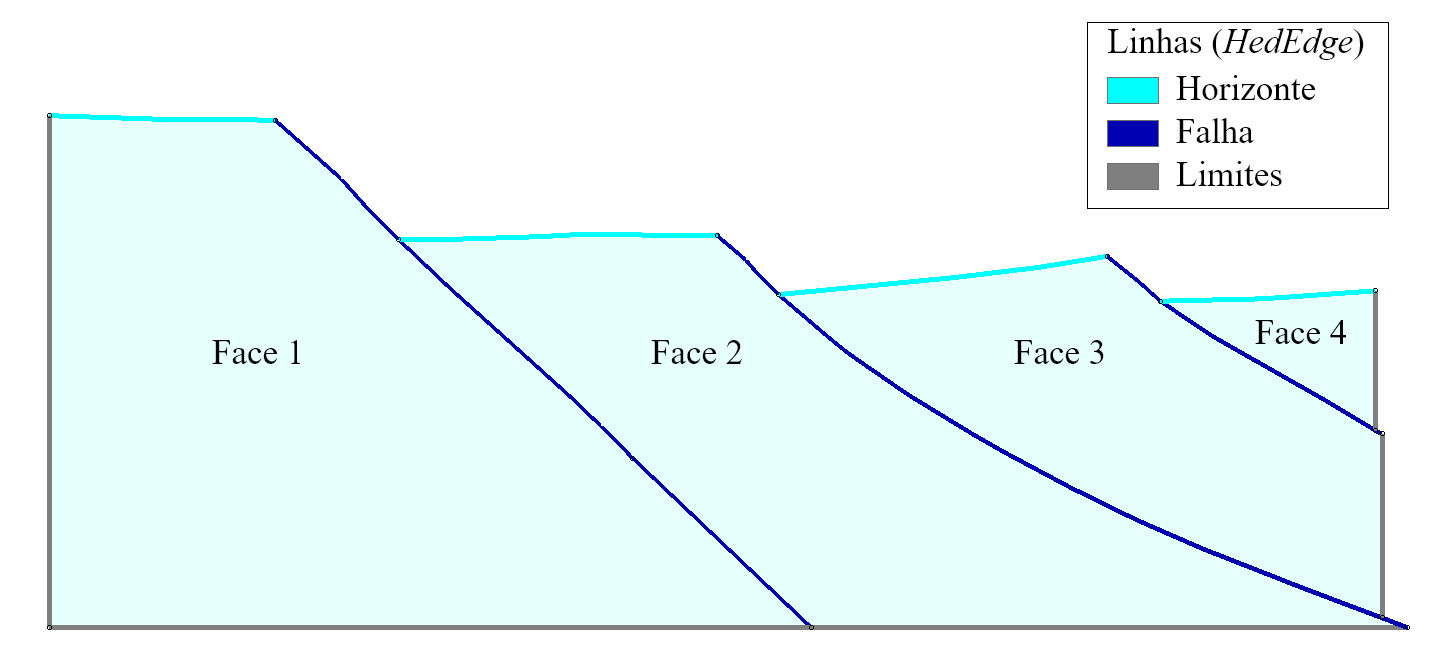
\includegraphics[width=\textwidth]{images/fig-recon-2}
    \caption{Seção geológica com destaque para os elementos de linhas e faces.}\label{fig-recon-2}
  \end{center}
\end{figure}

As faces têm um atributo muito importante para o trabalho de restauração, que são as malhas de triângulos. Cada face possui uma malha independente das outras. No Sistema Recon, essa malha é armazenada numa estrutura de dados topológicos chamada \textit{TopS} que trata-se de uma biblioteca computacional voltada para representação de malhas de elementos finitos.\cite{Tops} A Figura~\ref{fig-recon-3} exibe a mesma seção, mas com adição das malhas das faces.

\begin{figure} [H]
  \begin{center}
    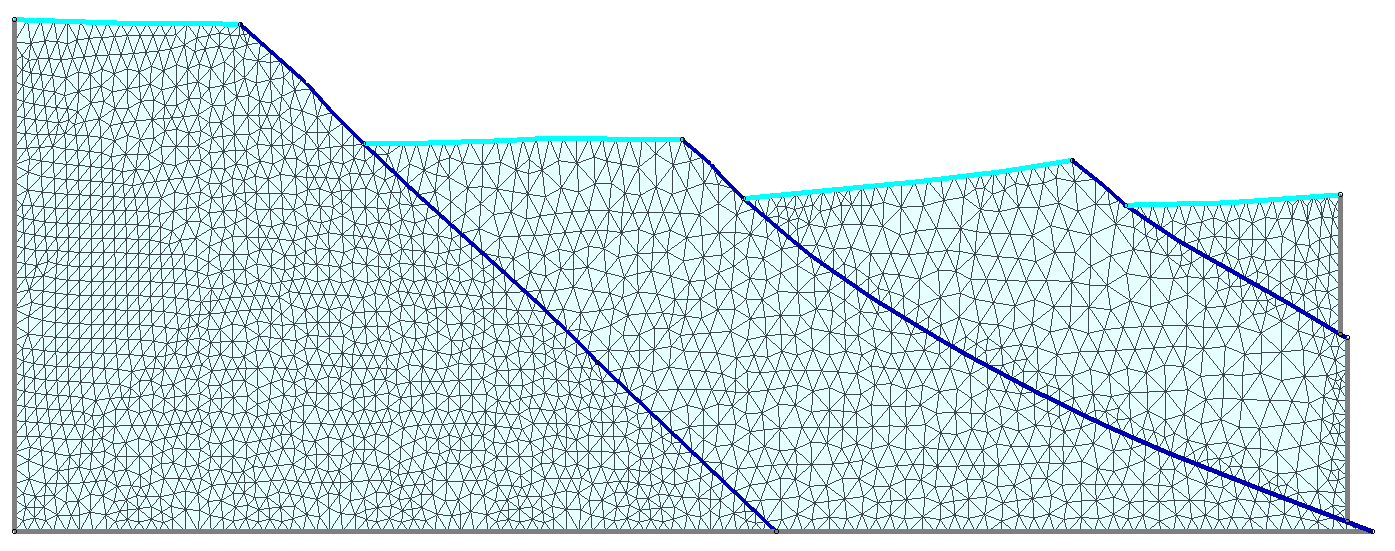
\includegraphics[width=350pt]{images/fig-recon-3}
    \caption{Malhas das faces de uma seção geológica no Sistema Recon.}\label{fig-recon-3}
  \end{center}
\end{figure}

A importância das malhas dentro da restauração de seções no Sistema Recon se dá por conta das transformações geológicas que possuem como requisito de entrada uma malha. Um pouco mais de detalhes sobre as transformações será apresentado adiante.

A estrutura \textit{TopS} permite armazenar certos atributos em seus elementos topológicos. Em especial nos vértices da malha, no Sistema Recon, é armazenado o \textit{UUID} do atributo geológico da entidade topológica do HED sobre a qual aquele vértice está, em outras palavras, se o vértice da malha está no interior da face, ele guarda o \textit{UUID} da \textit{GeoFace} dessa face, o mesmo para caso esteja sobre uma aresta (\textit{GeoEdge}) ou vértice (\textit{GeoVertex}). A Figura~\ref{fig-recon-4} mostra um exemplo da forma como esses dados são obtidos.

\begin{figure} [H]
  \begin{center}
    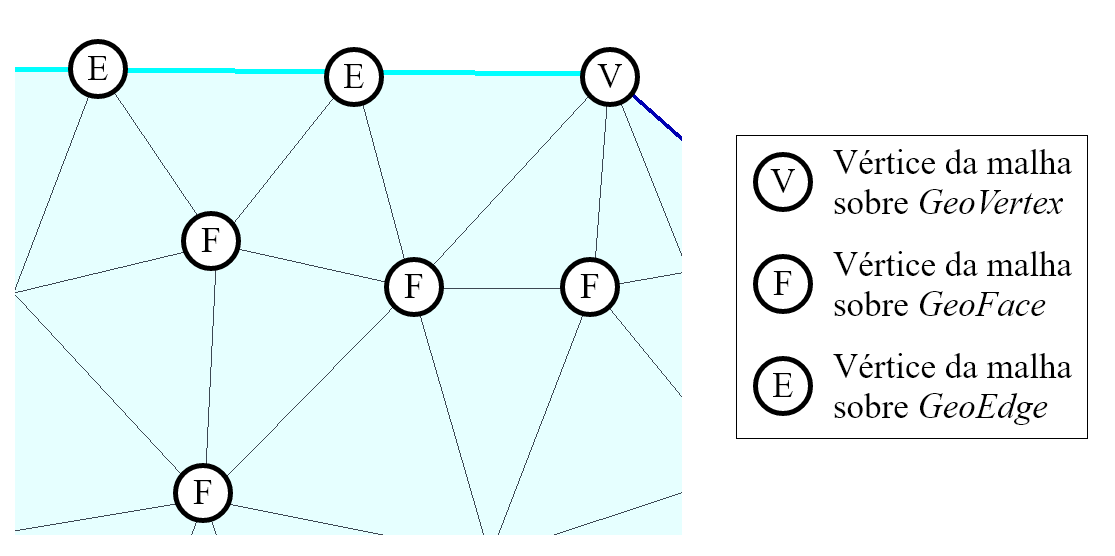
\includegraphics[width=\textwidth]{images/fig-recon-4}
    \caption{Trecho de uma malha de face com os tipos de atributo geológicos que estão sob os vértices da malha.}\label{fig-recon-4}
  \end{center}
\end{figure}

Essa relação permite identificar, a partir de um vértice da malha, sobre qual entidade geológica está este vértice, este recurso será usado no próximo capítulo.

\subsubsection{Transformações}

As transformações geológicas são ferramentas que buscam reverter (ou simular) as movimentações e deformações ocorridas aos blocos de rocha ao longo do tempo.\cite{Santi} As transformações são aplicadas diretamente às malhas, no entanto, para sua que isso aconteça, é necessário antes a definição de \textit{Módulos} na seção. 

Módulos nada mais são que agrupamentos de faces ou blocos da seção, têm o intuito de reunir aquelas partes que devem ter recebido as mesmas deformações, podendo ser, inclusive partes de camadas diferentes.

Com o módulo definido, consegue-se aplicar uma transformação. Esta irá ser empregada sobre a malha de cada uma das faces que compõem aquele módulo, deformando esta malha e, por conseguinte, alterar a geometria da seção.

A Figura~\ref{fig-recon-5} mostra a aba \quotes{Transformações} do Sistema Recon onde é possível ver os grupos de transformações e também a quantidade de opções disponíveis. Mais detalhes sobre cada uma delas podem ser consultados no manual do usuário do programa\cite{Recon}.

\begin{figure} [H]
  \begin{center}
    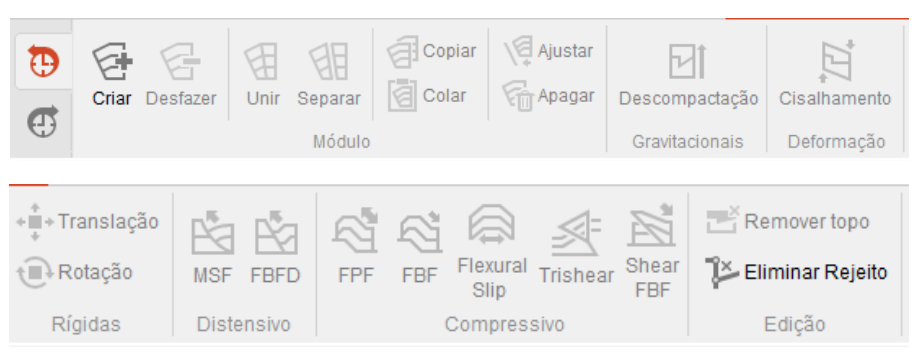
\includegraphics[width=\textwidth]{images/fig-recon-5}
    \caption{Aba \quotes{Transformações} do Sistema Recon.}\label{fig-recon-5}
  \end{center}
\end{figure}

\subsubsection{Árvore de cenários}

A restauração de seções é um processo linear no sentido de que cada novo passo depende de como estava o anterior e ainda por ser relacionado a uma escala de tempo, qualquer mudança num passo desses acarreta em um resultado diferente ao final. Além do mais, balanceamento de seções não é uma atividade de resposta única, dois geólogos podem chegar a resultados diferentes e igualmente corretos ao trabalharem com o mesmo modelo. 

Diante disto, o Sistema Recon disponibiliza em sua interface de manipulação das seções um componente capaz de registrar o histórico de etapas no processo de restauração, mais que isso, ao usuário é dado a possibilidade de voltar em algum ponto e criar uma nova linha de estudo dentro desse processo todo, ou ainda apagar uma sequência de etapas a que ele julga estar incorreta.

Isso tudo é possível graças à árvore de cenários. Um cenário é a representação de um estado de restauração de uma seção. Por exemplo, se de um passo a outro da restauração ocorre uma transformação, o estado anterior pode ser registrado em um cenário e o posterior em um outro. De cada cenário pode-se criar diversos outros como se fossem diferentes linhas do tempo, ou diferentes interpretações daquele passo de restauração.

Árvores são um tipo especial de estrutura de dados não-linear e neste casos de uso é definida como tendo uma raiz ou nó inicial que aponta para um ou mais outros nós. Estes, igualmente, podem apontar para outros diferentes nós numa escala hierárquica. A Figura~\ref{fig-recon-6} apresenta um exemplo de árvore de cenários tirada do Sistema Recon. Nesta imagem, cada quadrinho representa a seção num dado estado e como identificação, cada cenário também possui um número.

\begin{figure} [H]
  \begin{center}
    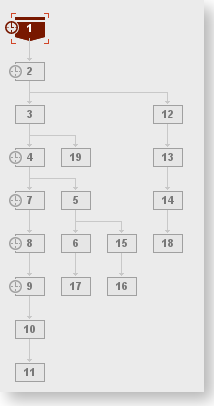
\includegraphics[width=160pt]{images/fig-recon-6}
    \caption{Exemplo de árvore de cenários de uma seção do Sistema Recon.}\label{fig-recon-6}
  \end{center}
\end{figure}

O primeiro cenário tem a seção em sua versão inicial e a cada nova manipulação da mesma, pode-se criar um novo cenário e assim ter este histórico. Essa maneira de organizar uma restauração é útil não só no contexto de uma seção isolada, mas principalmente quando se trabalha em modelos de multisseções que irão sofrer os mesmos processos de restauração, mas de maneiras diferentes. Com um registro do quê e quando ocorreu uma dada transformação em diferentes seções é possível ter uma visão mais geral do modelo em uma sequência cronológica.



\subsection{Etapas de restauração}



\subsection{Ambiente Multisseções}


  % -*- coding: utf-8; -*-

\chapter{Mapeamento}

O mapeamento descrito neste trabalho é baseado exclusivamente na restauração de seções geológicas. Para tanto, há necessidade de uma camada de informações proveniente das seções que contenha os dados a serem usados no mapeamento tridimensional. Essas informações podem ser extraídas com um tipo de mapeamento 2D presente nas seções, com o uso de \textit{linhas de mapeamento}.

Neste capítulo serão apresentados o conceito de linha de mapeamento presente no Sistema Recon, suas características, alguns casos de uso e também as derivações.

Após isso, haverá uma abordagem acerca dos procedimentos matemáticos e algoritmos computacionais presentes no mapeamento de superfícies e do volume, com inclusão de exemplos e discussão a respeito dos resultados obtidos em cada um.

\section{Linhas de Mapeamento}

Linhas de mapeamento são linhas formadas por \textit{pontos de mapeamento}. Estes pontos são objetos mapeados nas malhas da seção e guardam informação referente à sua localização dentro desta malha.

Um ponto de mapeamento, em razão dos tipos de entidades topológicas presentes na malha, pode ser do tipo nó, aresta ou elemento:

\renewcommand{\labelitemi}{•}
\begin{itemize}
  \item Nó: o ponto está sobre um nó da malha. É guardado o identificador desse nó.
  \item Aresta: caso onde o ponto localiza-se sobre uma aresta de elemento. Além do identificador da aresta, é armazenada a coordenada paramétrica do ponto.
  \item Elemento: o ponto encontra-se no interior de um elemento. Guarda-se o identificador do elemento e as coordenadas baricêntricas do ponto.
\end{itemize}

A criação dessas linhas se dá pela definição de uma linha-guia que pode cruzar diferentes regiões da seção. Para cada região interceptada, é criada uma parte de linha de mapeamento, essa parte armazena o identificador da malha da região. A interseção dos pontos da linha-guia com a malha produz os pontos de mapeamento.

A linha de mapeamento pode ser criada em qualquer cenário durante a restauração da seção e sua geometria pode ser calculada com base na malha em função dos pontos de mapeamento que a formam. Após a criação, uma versão da linha de mapeamento é gerada para cada cenário anterior e subsequente ao que foi usado na definição da linha-guia, é assim que 
ocorre o mapeamento dessa linha ao longo das etapas de restauração da seção.

O requisito para que seja calculada a geometria da linha em diferentes cenários é que a malha mantenha a mesma topologia, no entanto, mesmo em casos de edição, é possível realizar uma interpolação dos atributos presentes na malha para sua nova versão, incluem-se nisso as partes de linha de mapeamento que irão também receber uma nova versão equivalente dada a alteração na topologia da malha.

Dentro do Sistema Recon, a linha de mapeamento é um recurso importante na interpretação dos resultados gerados na restauração do modelo. Com ela é possível ter uma linha que acompanha a movimentação da malha de um cenário a outro.

As linhas de mapeamento (Figura~\ref{fig-linemap}) permitem realizar um mapeamento geométrico ao longo de uma restauração tomando como base uma linha-guia poligonal definida pelo usuário.

\begin{figure} [h]
  /\begin{center}
    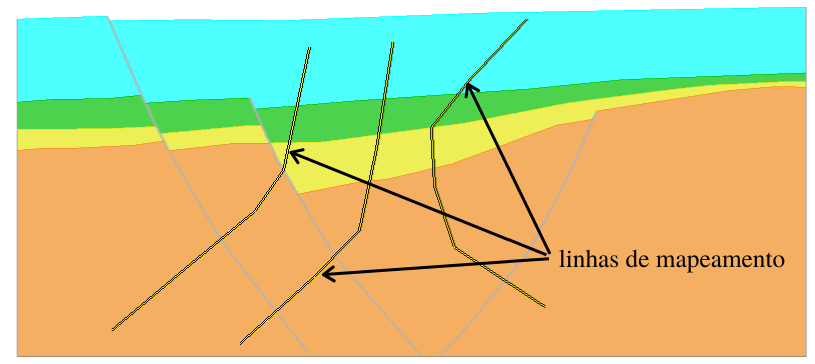
\includegraphics[width=400pt]{images/fig-linhas-de-mapeamento-ed}
    \caption{Linhas de mapeamento em uma seção.}\label{fig-linemap}
  \end{center}
\end{figure}

A Figura~\ref{fig-linemap-history} apresenta o resultado após uma transformação do tipo \textit{Move-Sobre-Falha} onde é possível observar, além da deformação da camada, a linha de mapeamento sofrendo a mesma movimentação. Este tipo de uso pode ser interpretado como se houvesse ali um falso horizonte para avaliar o quantidade de movimento na restauração do rejeito.

\begin{figure} [h]
  \begin{center}
    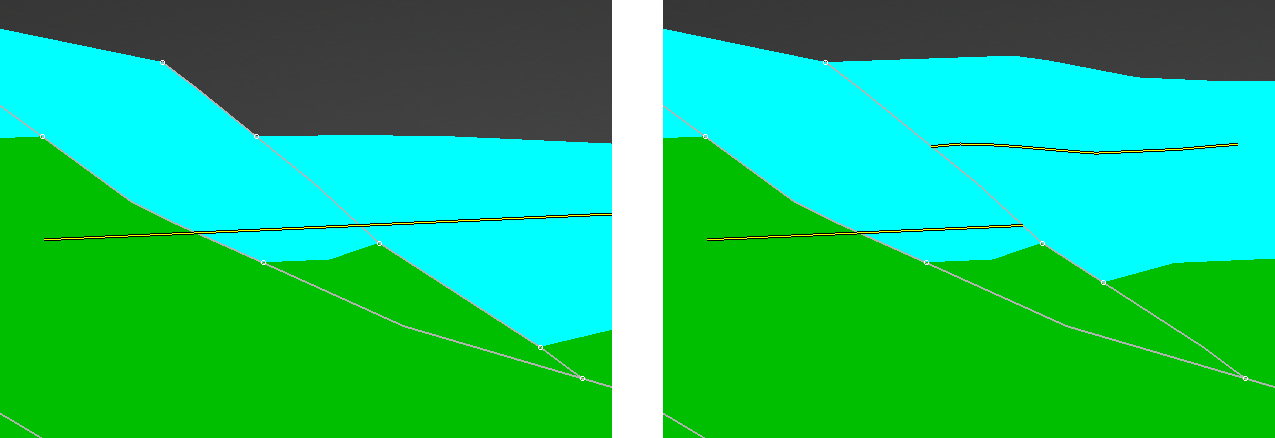
\includegraphics[width=420pt]{images/fig-linemap-history}
    \caption{Linhas de mapeamento em diferentes etapas}\label{fig-linemap-history}
  \end{center}
\end{figure}


O processo de criação da linha de mapeamento é feito para cada parte individualmente, de forma que ao visualizar as partes tem-se a linha de mapeamento completa. Na Figura~\ref{fig-linemap-malhas} é possível ver uma linha de mapeamento cortando algumas regiões diferentes.

\begin{figure} [h]
  \begin{center}
    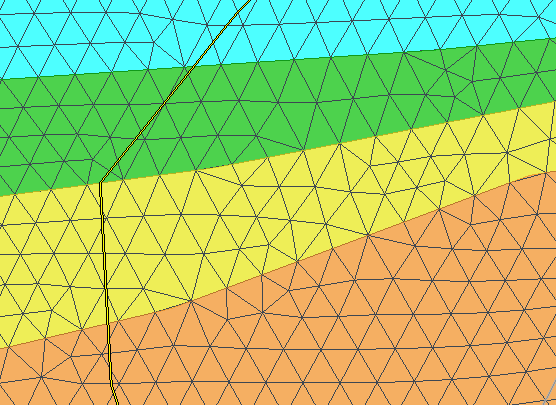
\includegraphics[width=250pt]{images/fig-linhas-de-mapeamento-malhas}
    \caption{Linhas de mapeamento cortando múltiplas faces.}\label{fig-linemap-malhas}
  \end{center}
\end{figure}

Na Figura~\ref{fig-linemap-parts} estão evidenciadas as partes que formam a linha de mapeamento. Como já dito, cada parte está associada à malha de um região diferente.

\begin{figure} [h]
  \begin{center}
    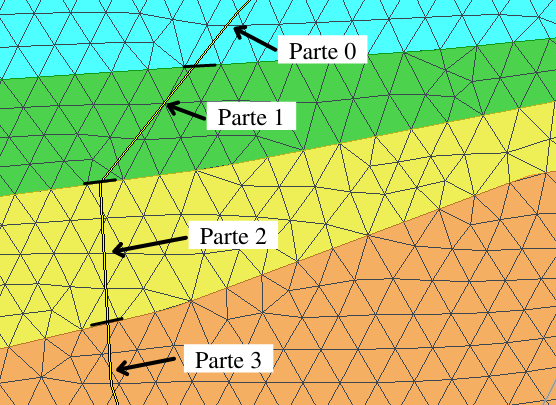
\includegraphics[width=250pt]{images/fig-lm-parts}
    \caption{Partes de uma linha de mapeamento}\label{fig-linemap-parts}
  \end{center}
\end{figure}

A Figura~\ref{fig-lm-topo} mostra a identificação dos pontos em uma parte de linha de mapeamento e a Tabela~\ref{tab-lm-topo} exibe quais informações topológicas são salvas de cada ponto.

\begin{figure} [hbt!]
  \begin{center}
    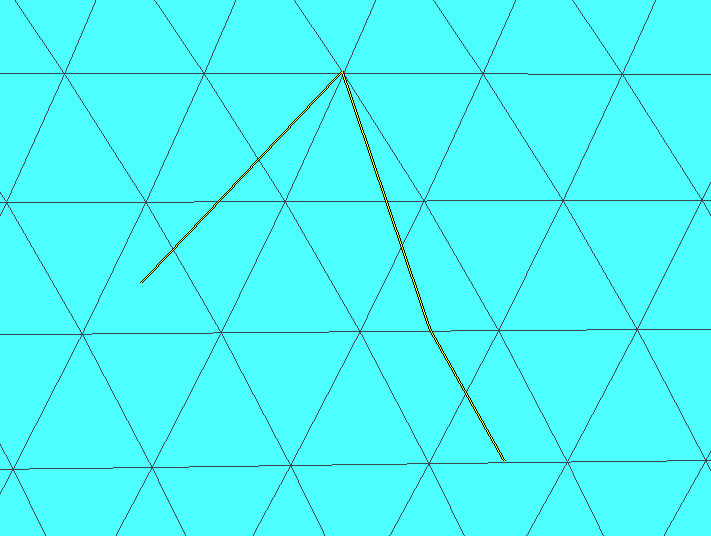
\includegraphics[width=260pt]{images/fig-lm-topo}
    \caption{Informações topológicas da malha mapeadas para a linha de mapeamento.}\label{fig-lm-topo}
  \end{center}
\end{figure}

% -*- coding: utf-8; -*-

\begin{table} [hbt!]
 \begin{center}
	 \caption{Informações topológicas salvas na linha de mapeamento.\label{tab-lm-topo}}
	~\\[-2mm]
	 \begin{tabularx}
		 {\textwidth}
		 {cp{2.0cm} lp{3.0cm} lp{10.0cm}}

		 \textbf{Ponto}
		 & \textbf{Tipo}
		 & \textbf{Informação armazenada} \\ \toprule

		 %~\\[-1mm]
		 A
		 & Elemento
		 & id=30, coordenadas baricêntricas=(0,33; 0,33; 0,33) \\ \midrule

		 %~\\[-1mm]
		 B
		 & Nó   
		 & id=431 \\ \midrule

		 %~\\[-1mm]
		 C
		 & Aresta
		 & id=130, coordenada paramétrica=0,45 \\ \midrule

		 %~\\[-1mm]
		 D
		 & Aresta
		 & id=145, coordenada paramétrica=0,55 \\ \midrule

	 \end{tabularx}
 \end{center}
\end{table}


\section{Derivações das Linhas de Mapeamento}

As linhas de mapeamento têm também casos de usos mais especializados dentro do Sistema Recon, como na criação e representação de poços. Poços são criados semelhantemente às linhas ou por importação de modelos com poços em 3D. Possuem característica de serem linhas quase verticalizadas e possuem uma finalidade mais limitada. Nos casos de poços 3D, a linha correspondente ao poço é apenas uma projeção do objeto tridimensional no plano da seção.

Há o uso nas chamadas linhas de interseção (\textit{CrossLine}) que servem para identificar e mapear as linhas de cruzamento entre seções no espaço tridimensional do multi-seções, com isso é possível ter uma noção do que ocorre com seções transversais mesmo estando no domínio bidimensional da restauração.

Por último, foi criada a \textit{linha de mapeamento do modelo} ou \textit{LMModel}, cujo objetivo é servir como um mapeamento das linhas que representam os elementos geológicas ao longo da restauração do modelo. Assim, é possível ter um acompanhamento do que ocorre com as entidades geológicas na seção, além de poder verificar como se deu a movimentação de cada ponto de horizonte, falha ou topo de sal ao longo da restauração.

As \textit{LMModels} são linhas de mapeamento baseadas no pontos do contorno da malha das regiões, ou seja, as partes que a formam possuem apenas pontos de mapeamento do tipo nó.

Pelo objetivo proposto, as \textit{LMModels} são linhas de mapeamento que tomam a geometria das entidades geológicas como entrada, então não há necessidade de criar uma linha-guia como é feita na linha de mapeamento original, a própria linha de horizonte, falha, ou topo de sal é usada como linha-guia.

Conforme o elemento geológico base, há um tipo de \textit{LMModel} e informações adicionais armazenadas:

\renewcommand{\labelitemi}{•}
\begin{itemize}
  \item Horizonte: é guardado a informação de idade deste horizonte.
  \item Falha: o identificador da falha é o dado armazenado.
  \item Topo de sal: apenas uma referência direta à linha original.
\end{itemize}

Todas essas informações  geológicas atreladas ao mapeamento topológico das \textit{LMModels}, quando em conjunto com as diversas seções geológicas de um modelo multi-seções, são o que fazem dela o principal dado para a realização de um mapeamento de informações de evolução do modelo tridimensional ao longo do tempo, já que trazem todo o histórico de movimentação das camadas de um modelo geológico.

A maneira de trabalhar com \textit{LMModels} é com a organização delas em estruturas de dados que formam subconjuntos divididos por etapa de restauração e idade (caso de linhas de horizonte). Com isso é obtido o conjunto de informações que representam a restauração das seções no Sistema Recon.

% Incluir exemplo de uma seção sem e com lmmodels

\section{Mapeamento de superfícies}

Na seção anterior foi apresentado um tipo de mapeamento bidimensional que é usado dentro da restauração de seções do Sistema Recon. Aqui será mostrado o mapeamento de superfícies baseado na restauração das seções que, neste trabalho, pode ser definido como o uso de informações das seções como parâmetros matemáticos para deformar os pontos da superfície e assim obter uma configuração coerente com a movimentação tectônica resultante das seções geológicas.

Essa deformação da superfície pode ser modelada como um problema variacional em termos de energia através de funções Lagrangeanas. A energia de superfície de membrana é uma PDE de segunda ordem, descrita pelo operador de Laplace $\Delta{q}$ e minimiza a área da superfície. A energia de placas-finas que minimiza a curvatura da superfície é descrita pela PDE de quarta ordem $\Delta^2{q}$. Já para minimização da variação da curvatura de superfícies pode ser usada uma PDE de sexta ordem, ou tri-harmônica, $\Delta^3{q}$, sua aproximação discreta é dita superfície de mínima variação.\cite{Muller, Botsch}





\subsection{Metodologia}

\subsection{Preparação dos dados}

\subsection{Exemplos e resultados}

\section{Mapeamento do Volume}

\subsection{Metodologia}

\subsection{Preparação dos dados}

\subsection{Exemplos e resultados}



  % -*- coding: utf-8; -*-

\chapter{Conclusão}

Assim, como uma proposta para trabalho futuro, pode-se buscar combinar
os dois enfoques...

  \arial
  \bibliography{tiny}
  \normalfont
  % -*- coding: utf-8; -*-

\appendix
\chapter{Published paper}

The following paper was published ...

\end{document}
